\documentclass{article}
\usepackage[spanish]{babel}

\usepackage[style=numeric,backend=bibtex8]{biblatex}
\addbibresource{./referencias.bib}

\usepackage{graphicx}
\usepackage{subfig}
\usepackage{caption}

\usepackage{amsmath}

\usepackage{listings}
\lstdefinestyle{CStyle}{
	basicstyle=\footnotesize,
	breakatwhitespace=false,
	breaklines=true,
	captionpos=b,
	keepspaces=true,
	numbers=left,
	numbersep=5pt,
	showspaces=false,
	showstringspaces=false,
	showtabs=false,
	tabsize=2,
	language=C
}

\renewcommand{\lstlistingname}{Código}

\title{Programación Orientada al Rendimiento.\\Proyecto de Programación Paralela.}

\author{Grupo 81\\ \\
	Gonzalo Juarez Tello, 100467578\\
	Hodei Urigoitia Merodio, 100374256\\
	Adrián Mancera González, 100429049\\
	Gonzalo Martinez Martín, 100428963
}

\date{}

\begin{document}

\begin{figure}
	
\includegraphics[width=\linewidth,height=0.7\textwidth]{resources/logo_uc3m.png}
\end{figure}
\maketitle
\newpage

\tableofcontents
\newpage

\section{Introducción.\label{intro}}
En esta parte de Programación Orientada al Rendimiento, paralelizamos
un programa simulador de fuerzas ejercidas entre objetos
en un cubo cerrado. Sobre este ejemplo estudiamos el impacto de las
estructuras de datos, los algoritmos, y las optimizaciones secuenciales
y paralelas en el rendimiento\footnote{rendimiento usado como sinónimo de
`tiempo de ejecución'.} final del programa.

Como refresco rápido repasamos primero el diseño secuencial en la sección \ref{original}.


En la sección \ref{opt} exploramos las optimizaciones tanto secuenciales como
paralelas que se tuvieron en cuenta. Haciendo comentarios
sobre cuales optimizaciones lograron permanecer en la versión final, cuáles no, y por qué es así.


Luego exponemos los resultados de las pruebas realizadas, los analizamos estadísticamente en la sección \ref{performance},
donde también cerramos con conclusiones al respecto.

\section{Diseño Original.\label{original}}
En el diseño original de este programa, ambas versiones SoA\footnote{Struct of Arrays} y AoS\footnote{Array of Structs}
son bastante similares. Por lo que consideramos que en este repaso no vale la pena discutir sus diseños por separado.


Una vez superada la inicialización de los objetos. Ambas versiones consisten en 3 loops anidados.
Un loop externo (con variable \textit{k} de manera que $0\leq{k} < {num\_iterations}$),
un loop interno que itera por todos los objetos de uno en uno usando una variable \textit{i}
($0\leq{i} < {num\_objects}$), y un loop externo que itera por los objetos desde \textit{i}
excluyendo \textit{i} ($i+1\leq{j} < {num\_objects}$).

A lo largo de la memoria, a esta última
parte de los loops anidados con variables \textit{i} y \textit{j} le llamaremos \textbf{doble loop} ó \textbf{loop doble}.
Su forma básica puede verse en Código \ref{doble_loop:no_striping-no_tiling}.
Es una estructura recurrente en el programa. La variable k desde el vamos no se presta a optimizar porque
necesita la verificación de colisiones antes de cada iteración (tiene una dependencia de datos total
entre una iteración y la otra). El doble loop aparece tanto en verificación de colisiones, como en cálculo de
fuerzas resultantes de un objeto con el resto.


En cada loop doble se calculan las fuerzas resultantes de un objeto con todos los demás, se añade la
correspondiente fuerza resultante a cada cuerpo involucrado en el cálculo, y luego se calcula la
aceleración, velocidad, y nueva posición del objeto \textit{i}. La optimización más importante de la
versión original (y la más obvia) es esta de evitar calcular dos veces la fuerza resultante entre
dos objetos. Esto resulta en un espacio de iteración triangular. La forma del espacio de iteración nos es de mucho interés
a la hora de tener en cuenta optimizaciones (sección \ref{opt}). La figura \ref{fig:no_tiling} ilustra
el espacio de iteración del doble loop, así como su flujo de ejecución.


Por último, el diseño original nunca elimina objetos, si no que
los marca. Luego en el código hay condicionales para poder
ignorar aquellos objetos marcados como eliminados.

\begin{lstlisting}[style=CStyle,label=doble_loop:no_striping-no_tiling,caption=doble loop simple.]
for (i = 0; i <= N; ++i)
	for (j = i+1; j <= N; j++)
\end{lstlisting}

\begin{figure}[h!]
	\centering
	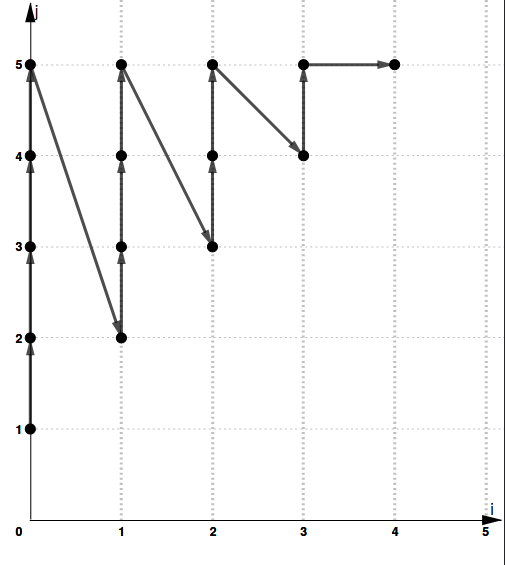
\includegraphics[width=0.6\linewidth,height=0.6\textwidth]{resources/loop_anidado_no_tiling_505x565.png}
	\caption{espacio de iteración de $0\leq{i} < {N}$, y $i+1\leq{j} < {N}$
	cuando ${N}=5$, y N se corresponde al número de objetos. Las flechas marcan el flujo de ejecución del loop doble.
	delimitado por las flechas. \textit{i} en eje de abscisas, \textit{j} en eje de ordenadas.}
	\label{fig:no_tiling}
\end{figure}
%\newpage

\section{Optimizaciones.\label{opt}}

En esta sección discutimos distintas optimizaciones, su impacto en la performance,
y su impacto en los resultados. El tratar con operaciones en punto flotante, el programa
lidia con un trade-off entre precisión en los resultados y mejoras tiempo de ejecución.

\subsection{Optimizaciones secuenciales.\label{opt_seq}}
Las siguientes optimizaciones no solamente intentan mejorar la velocidad
del código de ejecución serializada. Si no también preparar al algoritmo
para poder aprovechar mejor la paralelización a nivel de tarea.

\subsubsection{Vectorización en cálculos de fuerza.\label{simd}}
El título de la subsección \ref{opt_seq} habla de optimizaciones secuenciales, pero hay un poco de mentira
en ese título. El paralelismo a nivel de datos puede dar mejoras de rendimiento a aplicaciones
que procesen grandes conjuntos de datos (similar a nuestro programa). Las distintas familias de instrucciones
\textbf{SIMD}\footnote{Single Instruction-Multiple Data} que disponen las arquitecturas x86-64 son
ejemplos de paralelismo a nivel de datos. Estas operaciones son capaces de aplicar la misma operación sobre varios
datos al mismo tiempo.

En nuestro código intentamos sacar ventaja de esto, pero la \textit{vectorización} tiene algunos requisitos \cite{intel_vec_guidelines}.
Evitar dependencias de datos, especialmente de tipo RAW. Y ausencia de estructuras condicionales a no ser
que puedan ser tratadas como \textit{masked assignments}. Otras operaciones simplemente no son vectorizables
en su manera ``pura''(un ejemplo es sqrt()\footnote{sqrt() es vectorizable si se indica \textit{-funsafe-math-optimizations},
en tiempo de compilación. Pero a cierto punto, el error propagado es muy grande (como se menciona en \ref{compiler})}).


El diseño original tiene condicionales dispersos por todo el código. Como se menciona en
la sección \ref{original}, los objetos no se eliminan, se marcan, y se debe verificar su existencia.
Todo esto lo hace la función de chequeo de colisiones. Si esta función se divide en una parte de marcado
de colisiones y fusión de objetos (que no hace más que sumar objeto \textit{a} con objeto \textit{b}), y
una segunda parte donde se eliminen en una sola pasada los objetos marcados y se actualice la longitud
del array de objetos. Entonces el resto del código no necesita condicionales para verificar la existencia de objetos.


Otra restricción para que el compilador pueda vectorizar el código, es la \textit{supresión de dependencias de datos}.
En particular y como mínimo, evitar \textit{RAW} (al menos en x86-64). El cálculo de fuerzas tiene este tipo de dependencias en algunas
partes. Por ejemplo, el objeto en el índice del loop menos profundo \textit{i}, tiene dependencias WAW entre iteraciones.
O bien, hay dependencias RAW propias de utilizar el resultado de un cálculo almacenado en una variable para un nuevo cálculo.


La técnica \textit{strip-mining} (presentada en \ref{strip-mining}) expone la vectorización
del algoritmo, y ayuda a eliminar algunas dependencias WAW (al convertir variables únicas en arrays). No es
la única utilidad que se le da en el programa final a esta técnica, pero en esta sección es lo que nos importa.


Para lidiar con RAW, una posible solución es la de dividir un loop con RAW en 2 loops sin RAW (también
facilitado por strip-mining). Pero esto puede resultar en una pérdida de rendimiento, por lo tanto
hay que medir la performance del programa.


El código original no pareció incorporar muy bien las instrucciones SIMD en el cálculo de fuerzas.
Por alguna razón (que no pudimos determinar analizando el código fuente)
incluso eliminando las dependencias de datos, el compilador se rehúsa a vectorizar
una parte caliente\footnote{parte del programa accedida con mucha frecuencia} del código. Obligar la vectorización
con la directiva \textit{\#pragma omp simd} no termina en buenos resultados ni performance (claramente el compilador
es más inteligente).

\subsubsection{Strip-mining.\label{strip-mining}}
Strip-mining es una técnica que expone oportunidades de vectorización al compilador, como es mencionado
en la subsección \ref{simd}. Varias veces el compilador puede llevar a cabo esta optimización por su cuenta.


También puede mejorar la localidad tanto espacial como temporal si los mismos datos son utilizados en distintas partes
del algoritmo. Este último uso es el que se le dá en la versión final del código para el cálculo de fuerzas.


Si N es el tamaño del array a recorrer, se utiliza un tamaño de \textit{stride} ó \textit{step} para que una variable \textit{ii}
tome valores $0\leq{ii}\leq N$ avanzando cada iteración el valor del step. Luego la variable \textit{i} original puede recorrer
el tamaño de \textit{stride} de uno en uno. Esto aplicado a \textit{loop doble}, lo deja expresado de como se lo ve en
Código \ref{doble_loop:striping-no_tiling}.

Es importante aclarar que strip-mining por sí solo no altera el orden de ejecución del programa. Por lo
que el gráfico de Figura \ref{fig:no_tiling} sigue aplicando.

\begin{lstlisting}[style=CStyle,label=doble_loop:striping-no_tiling,caption=doble loop con strip-mining en ambos loops.]
/* strip-mining de cabecera de loop 1 */
for (ii = 0; ii <= N; ii+=stride)
for (i = ii; i <= min(ii+stride-1, N); ++i)
	/* strip-mining de cabecera de loop 2 */
	for (jj = i+1; jj <= N; jj+=stride)
	for (j = jj; j <= min(jj+stride-1, N); j++)
\end{lstlisting}


El código final también hace uso de la técnica para evitar false-sharing, algo que se explica con mas profundidad
en \ref{strip-mining-parallel}, la sección de esta técnica en las optimizaciones paralelas.

\subsubsection{Loop-tiling en loops anidados.\label{loop-tiling}}

Loop-tiling es una técnica para mejorar la localidad temporal en loops anidados de
n-dimensiones\footnote{profundidad del anidado de loops}. A su vez, caba bloque resultante
es un buen candidato como unidad de trabajo para la paralelización de tareas, disminuyendo
la frecuencia de sincronización. El tamaño de cada bloque puede
cambiarse para aprovechar la localidad propuesta por la jerarquía de memoria. Y la vectorización
se asienta naturalmente dentro de un bloque \cite{Wolfe89moreiteration}.


Básicamente consiste en 2 pasos: strip-mining, y permutación loops.


Strip-mining es el primer paso para loop-tiling. Ya está cubierto en la subsección \ref{strip-mining}.


El último paso, la permutación o intercambio de loops \textit{simplemente}, consiste en cambiar las cabeceras de los bucles.
Esto es válido cuando las dependencias de datos no existen o se mantienen lexicográficamente positivas
tras el intercambio de loops \cite{Laforest10ece1754}.


Asumiendo que los loops son independientes (que en nuestro caso, de asumir asociatividad, lo son),
¿qué tan simple es el intercambio de loops? En un espacio de iteración cuadrado, bastante simple. Resulta
que es un poco más complicado de lo que parece. De la sección \ref{original} entendemos que
nuestro espacio de iteración es triangular (como se lo ve en la figura \ref{fig:no_tiling}).
En un loop como el de Código \ref{doble_loop:striping-no_tiling}, nos gustaría permutar las cabeceras de manera que
\textit{ii} y \textit{jj} sean las primeras 2 cabeceras, con el loop de \textit{i} por debajo, y finalmente
el de \textit{j}. Para lograr esto hay que permutar la cabecera del loop \textit{i} con la del loop \textit{jj}.


¿Cómo implementar loop-tiling en un espacio de iteración triangular? El \textbf{modelo del poliedro} es parte
de un área de estudio que lleva bastante tiempo siendo desarrollada. Básicamente plantea que los espacios
de iteración que puedan ser pensados como un \textbf{poliedro convexo}\footnote{convexo: una línea entre 2 puntos
del poliedro pasa únicamente por puntos interiores al poliedro} (como un espacio triangular) y cumplan las dependencias
de datos previamente explicadas, pueden replantearse para intercambiar cabeceras. La metodología consiste en
plantear un sistema de inecuaciones que defina al \textbf{poliedro S} a partir de las cláusulas de los loops. Luego utilizar
el \textbf{método de eliminación de Fourier-Motzkin} para proyectar la variable a reacomodar (o sea, variable a eliminar y
reinsertar en algún momento). Tras la proyección, un sistema de inecuaciones de n-dimensiones (loop de n-variables)
queda como un sistema de m-dimensiones donde $m=n-1$. Con el método de Fourier-Motzkin se pueden eliminar progresivamente las variables,
para finalmente reinsertar las cabeceras de dichas variables eliminadas, bajo las nuevas cláusulas (inecuaciones). Este resultado
final es un nuevo sistema de inecuaciones que define un \textbf{poliedro S'} tal que \textit{S' es equivalente a S}.
Esta conversión en nuestro \textbf{doble loop} se representa como en la Figura \ref{fig:fourier_motzkin}. El código
resultante para las cabeceras es el de Código \ref{doble_loop:striping-tiling}.


Tanto el modelo del poliedro como la eliminación por método de Fourier-Motzkin, tienen utilidades más allá
de estas optimizaciones.

\begin{figure}
\begin{displaymath}
	\begin{array}{rrr}
		S\begin{cases}
			ii\geq 0\\
			ii\leq n\\
			i\geq ii\\
			i\leq n\\
			i\leq ii+stride-1\\
			jj\geq i+1\\
			jj\leq n\\
			j\geq jj\\
			j\leq jj+stride-1\\
			j\leq n
		\end{cases}
		&
		\textit{equivalente a}
		&
		S'\begin{cases}
			ii\geq 0\\
			ii\leq n\\
			i\geq ii\\
			i\leq n\\
			i\leq ii+stride-1\\
			jj\geq ii+1\\
			jj\leq n\\
			j\geq jj\\
			j\geq i+1\\
			j\leq jj+stride-1\\
			j\leq n\\
		\end{cases}
	\end{array}
\end{displaymath}
	\caption{Pasaje del sistema de inecuaciones que define al poliedro \textit{S} en Código \ref{doble_loop:striping-no_tiling},
	al sistema de inecuaciones que define al poliedro \textit{S'} en Código \ref{doble_loop:striping-tiling}. Notar
	como las condiciones en las cabeceras de Código \ref{doble_loop:striping-no_tiling} y \ref{doble_loop:striping-tiling} se corresponden
	de manera directa con los sistemas de inecuaciones \textit{S} y \textit{S'}, respectivamente.}
	\label{fig:fourier_motzkin}
\end{figure}

\begin{lstlisting}[style=CStyle,label=doble_loop:striping-tiling,caption=doble loop con loop-tiling.]
for (ii = 0; ii <= N; ii+=stride)
for (jj = i+1; jj <= N; jj+=stride)
	for (i = ii; i <= min(ii+stride-1, N); ++i)
		for (j = max(jj, i+1); j <= min(jj+stride-1, N); j++)
\end{lstlisting}

\begin{figure}[h!]
	\centering
	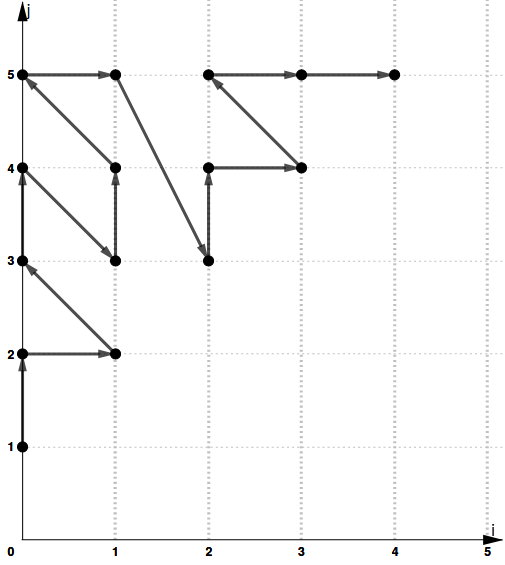
\includegraphics[width=0.6\linewidth,height=0.6\textwidth]{resources/loop_anidado_tiling_505x565.png}
	\caption{espacio de iteración triangular con loop-tiling cuando $N=5$ y $stride=2$. Flujo de ejecución
	delimitado por las flechas. \textit{i} en eje de abscisas, \textit{j} en eje de ordenadas.}
	\label{fig:no_tiling}
\end{figure}


Esta optimización en conjunto con vectorización (sección \ref{simd}) dieron al programa un speedup de más de x2.
A mayor número de objetos e iteraciones, mayor la diferencia con el código original, no porque el optimizado se
vuelva más rápido, si no porque el original debe reemplazar todos los datos en caché por cada iteración del loop \textit{j},
aumentando el speedup de la versión vectorizada con loop-tiling para esa configuración.


Pero asumir asociatividad en las operaciones de punto flotante no pudo contener la propagación del error
para número de objetos e iteraciones grandes ($N > 4000$, $iteraciones > 250$), por lo que loop-tiling fue descartado
como optimización tanto para el cálculo de fuerzas como para el marcado de colisiones. No obstante hay un único loop del cálculo de fuerzas que pudo mantenerse vectorizado para conseguir un muy pequeño, pero
mesurable, speedup.

\subsubsection{Flags de compilador.\label{compiler}}
Como programadores, además de jugar con el algoritmo, podemos jugar con las flags
del compilador en este trade-off de performance por precisión y viceversa.
Las flags usadas son:
\begin{itemize}
		\item -O3
		\item -fexcess-precision=fast -fno-rounding-math -fno-signaling-nans
			-fno-math-errno -fno-signed-zeros -fno-trapping-math: Son algunas de las optimizaciones
			sobre punto flotante que son activadas por -ffast-math. Pero -ffast-math
			a su vez activa -funsafe-math-optimizations (aproximación por métodos numéricos, multiplicación por inverso, y asociatividad
			de punto flotante, entre otras cosas). A cierto número de objetos e iteraciones, el error
			de -funsafe-math-optimizations se propaga demasiado. En cambio, estas otras flags no muestran cambios en el resultado porque, en su
			mayoría, son para señalizar errores como por ejemplo división por cero. Lo cual, si la detección
			de colisiones funciona bien, no debería pasar.
		\item march=native: optimizaciones especificas para la arquitectura que compile el programa (en el procesador
			utilizado esto resulta en vectorización por AVX y AVX512 en lugar de SSE).
\end{itemize}

\subsection{Optimizaciones con paralelismo.\label{opt_parallel}}
\subsubsection{Paralelismo en cálculos de fuerza y verificación de colisiones.}
La mayoría de las optimizaciones en paralelismo se enfocan alrededor del cálculo de fuerza resultante.
Esta parte del programa es la que ocupa la mayor parte del tiempo de ejecución. Y al tratarse de una sumatoria,
con cuidado por el punto flotante, es donde podría conseguirse un speedup significativo.


Inicialmente se intentó aprovechar al máximo las técnicas de loop tiling y vectorización discutidas
en \ref{loop-tiling} y \ref{simd}. El speedup de estas 2 técnicas sin paralelizar ya era alto, y en
papel (y cometiendo el grave error de ignorar de asumir asociatividad), el mismo algoritmo es muy apto a ser paralelizable.
Se paralelizó tanto del loop de \textit{ii} como el de \textit{jj} (por separado, sin directiva `collapse' ni colapso manual),
sumado a la paralelización y loop-tiling del loop para marcado de colisiones. El tiempo de ejecución para 10000 objetos, 500 iteraciones y un
tamaño de recinto de $10^6$ era de alrededor de 22 segundos para el código optimizado de manera secuencial y paralela,
una diferencia de poco más de 200 segundos al comparar con el tiempo de ejecución del programa secuencial de la sección \ref{original}.
Aunque se usaron técnicas de reducción para evitar carreras de datos y false-sharing, esto resultó en muchas operaciones
no asociativas ocurriendo desordenamdamente por la naturaleza misma del algoritmo. No solo eso, si no que
por depender del scheduler del sistema operativo (no se usaron directivas de ordenamiento), el resultado era no determinístico.


En la versión final del código únicamente se paraleliza el loop de cabecera \textit{jj}, obtenido
por strip-mining, no por loop-tiling (similar a Código \ref{doble_loop:striping-no_tiling}).
Loop-tiling desordena las operaciones para mejorar su localidad temporal.


El bucle \textit{jj} tiene una directiva de ordenamiento (`\#pragma omp ordered'), y en su interior
no hay un bucle \textit{j}, si no tres\footnote{una de las ventajas de strip-mining: rehúso de un mismo dato en distintas partes
del algoritmo}:

\begin{enumerate}
	\item El primero de estos loops \textit{j} no es vectorizable sin perder precisión ya que usa la función \textit{sqrt()} para
obtener la norma.

	\item El segundo loop calcula un factor común al cálculo de fuerzas en todas las componentes, o sea, evita
recalcularlo. Esto asume algo de asociatividad, pero no afecta los resultados numéricos con relación al programa original.
Además, este segundo bucle \textit{j} es la única parte vectorizable del cálculo de fuerzas, ya que por alguna razón el
cálculo de fuerzas resultantes y su posterior adición a los objetos en una reducción, cambia los resultados. Sin embargo,
esta pequeña vectorización otorga un speedup pequeño pero hace una diferencia en fin.


	\item Finalmente, el último bucle \textit{j} funciona como reducción y tiene en su cabecera la directiva de ordenamiento
necesaria por \textit{OpenMP} para forzar el orden de ejecución.

\end{enumerate}

\subsubsection{Uso de Strip-mining para paralelismo.\label{strip-mining-parallel}}
Strip-mining en paralelismo facilita la división la tarea en tiras del tamaño \textit{stride}, de la misma
manera en que los bloques generados por loop-tiling son la unidad de trabajo candidata para la división
de tareas \cite{Wolfe89moreiteration}. Con esto y ayuda del parámetro de directiva \textit{schedule} de \textit{OpenMP},
se reducen las condiciones de carrera, el exceso de sincronización, y \textit{cache-thrashing}\footnote{cantidad excesiva
de fallos a caché por múltiples núcleos intentando accediendo a la misma dirección de memoria.}.

Esto último es confirmado por las mediciones de fallos a caché de la herramienta \textit{perf c2c}.
Donde los fallos a caché privada con strip-mining se mantienen por debajo o alrededor de 3\%
(dependiendo de la configuración de la ejecución). Porcentaje de fallos que se hace notar en
el tiempo de ejecución al comparar con su contraparte sin strip-mining.


\subsection{Conclusiones sobre las optimizaciones.\label{opt_conclusiones}}
Asumir asociatividad de punto flotante es un error que solo pueden permitirse iteraciones
y números de objetos bajos. Intentar implementar aunque sea en pequeñas partes del código algunas de
las optimizaciones presentadas terminaban en un cambio de resultados. Alteraciones del orden de operaciones
en el espacio de iteración triangular, vectorización, y flags del compilador, fueron las principales
variables a controlar para poder mantener los resultados de la primera versión.


A continuación se exponen los resultados numéricos de las pruebas realizadas.
Desde ya, con tanta limitación a la hora de optimizar, el algoritmo paralelo no difiere mucho del
original de la sección \ref{original}.

\section{Evaluación de Rendimiento.\label{performance}}
El multiprocesador donde se desarrolló el código y se ejecutaron las pruebas es un
procesador intel i7 de 10ma generación, modelo \textbf{i7-1065G7}:
\begin{itemize}
	\item 4 núcleos (8 hilos).
	\item caché L1 de datos: 192 KiB (48 KiB por núcleo), 12 vías (64 conjuntos por núcleo), línea de caché de 64 bytes.
	\item caché L1 de instrucciones: 128 KiB (32 KiB por núcleo), 8 vías (64 conjuntos por núcleo), línea de caché de 64 bytes.
	\item caché L2 privada: 2 MiB (512 KiB por núcleo), 8 vías (1024 conjuntos por núcleo), línea de caché de 64 bytes.
	\item caché L3 compartida: 8MiB, 16 vías (8192 conjuntos), línea de caché de 64 bytes.
\end{itemize}
El sistema operativo usado es la distribución de \textbf{Linux OpenSUSE Tumbleweed} (rolling-release),
bajo el \textbf{kernel 5.15.x}. El compilador es \textbf{GCC 11.2.x}, ofrecido por el repositorio de OpenSUSE.

\subsection{Resultados obtenidos.}
Para las pruebas hemos estudiado la configuración con parámetros fijos ${size\_enclosure}=10^5$ ${random\_seed}=666$ y
${time\_step}=0.1$. En los parámetros restantes, representados en la tupla $({num\_objects}, {num\_iterations})$,
estudiamos las combinaciones $(4000, 250)$, $(4000, 500)$, $(8000, 250)$, y $(8000, 500)$. Por lo que hay
un total de 4 pruebas por configuración.

Cada prueba tiene una muestra de tamaño ${n}=10$. Estadísticamente
hablando, una muestra tan pequeña ($n < 30$) no nos permite aprovechar el \textit{Teorema del Límite Central}.
Por lo que las pruebas de comparación de 2 medias por distribución normal de dos colas, y ANOVA\footnote{Análisis de Varianza}
no han sido utilizadas. En su lugar, se optó por \textbf{T-Test} para la comparación de dos medias, y se reemplazó a ANOVA
por su equivalente no paramétrico: \textbf{Kruskal-Wallis H-Test}.

\subsection{Todos contra todos.\label{kruskal}}
En esta primera comparación buscamos las diferencias, si las hay en tiempos de ejecución para el programa
paralelo con diferentes cantidad de hilos de ejecución, y el programa secuencial. En particular, se comparan
los tiempos de ejecución para las 4 configuraciones de las pruebas en el programa secuencial y en el programa paralelo
con 16, 8, 4, 2, y 1 hilo de ejecución.


Para no rellenar páginas con gráficos, las figuras \ref{fig:8core_p_1} y \ref{fig:4core_16core} muestran únicamente los casos de 4, 8 y 16 hilos de ejecución, así como los resultados del programa
secuencial bajo la misma carga, usando la estructura de datos \textit{SoA}. Estos casos son suficientes
para un análisis comprensivo de SoA en las secciones \ref{kruskal} y \ref{t-test}.


En esta primera prueba, como fue mencionado ya, usamos la prueba no paramétrica de \textit{Kruskal-Wallis}. Planteando
las hipótesis alternativa y nula correspondientes:
\begin{displaymath}
\begin{cases}
	{H_0}: \text{las medias poblacionales son iguales.}\\
	{H_A}: \text{al menos una media poblacional difiere.}\\
\end{cases}
\end{displaymath}
\begin{figure}[htp]
	%\centering
	\hspace*{-3.5cm}
	\subfloat[Pruebas con 8 hilos de ejecución.]{%
		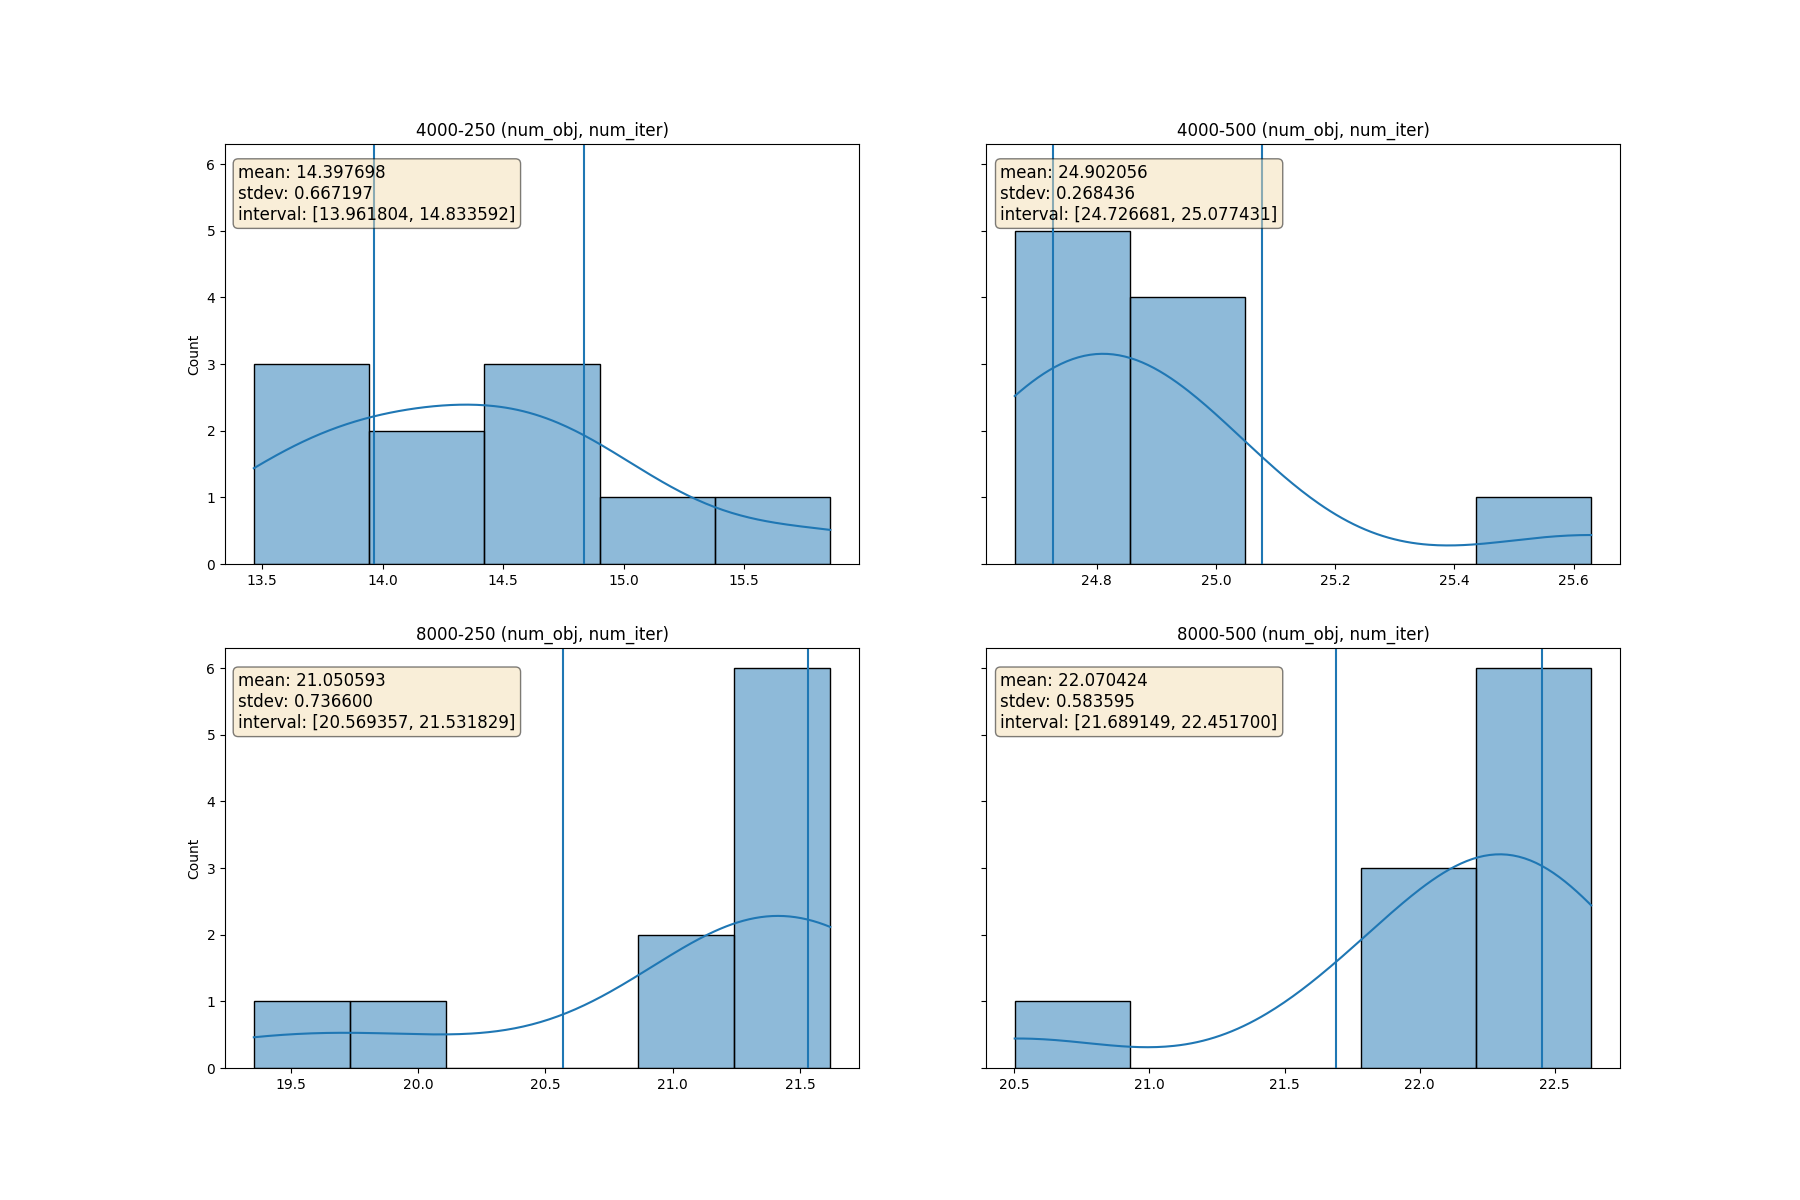
\includegraphics[width=0.8\linewidth,height=0.55\linewidth]{resources/8core_samples_conf_interval.png}
		\label{fig:8core}
	}%
	%\hfill%
	\subfloat[Pruebas en algoritmo secuencial de la sección \ref{original}.]{%
		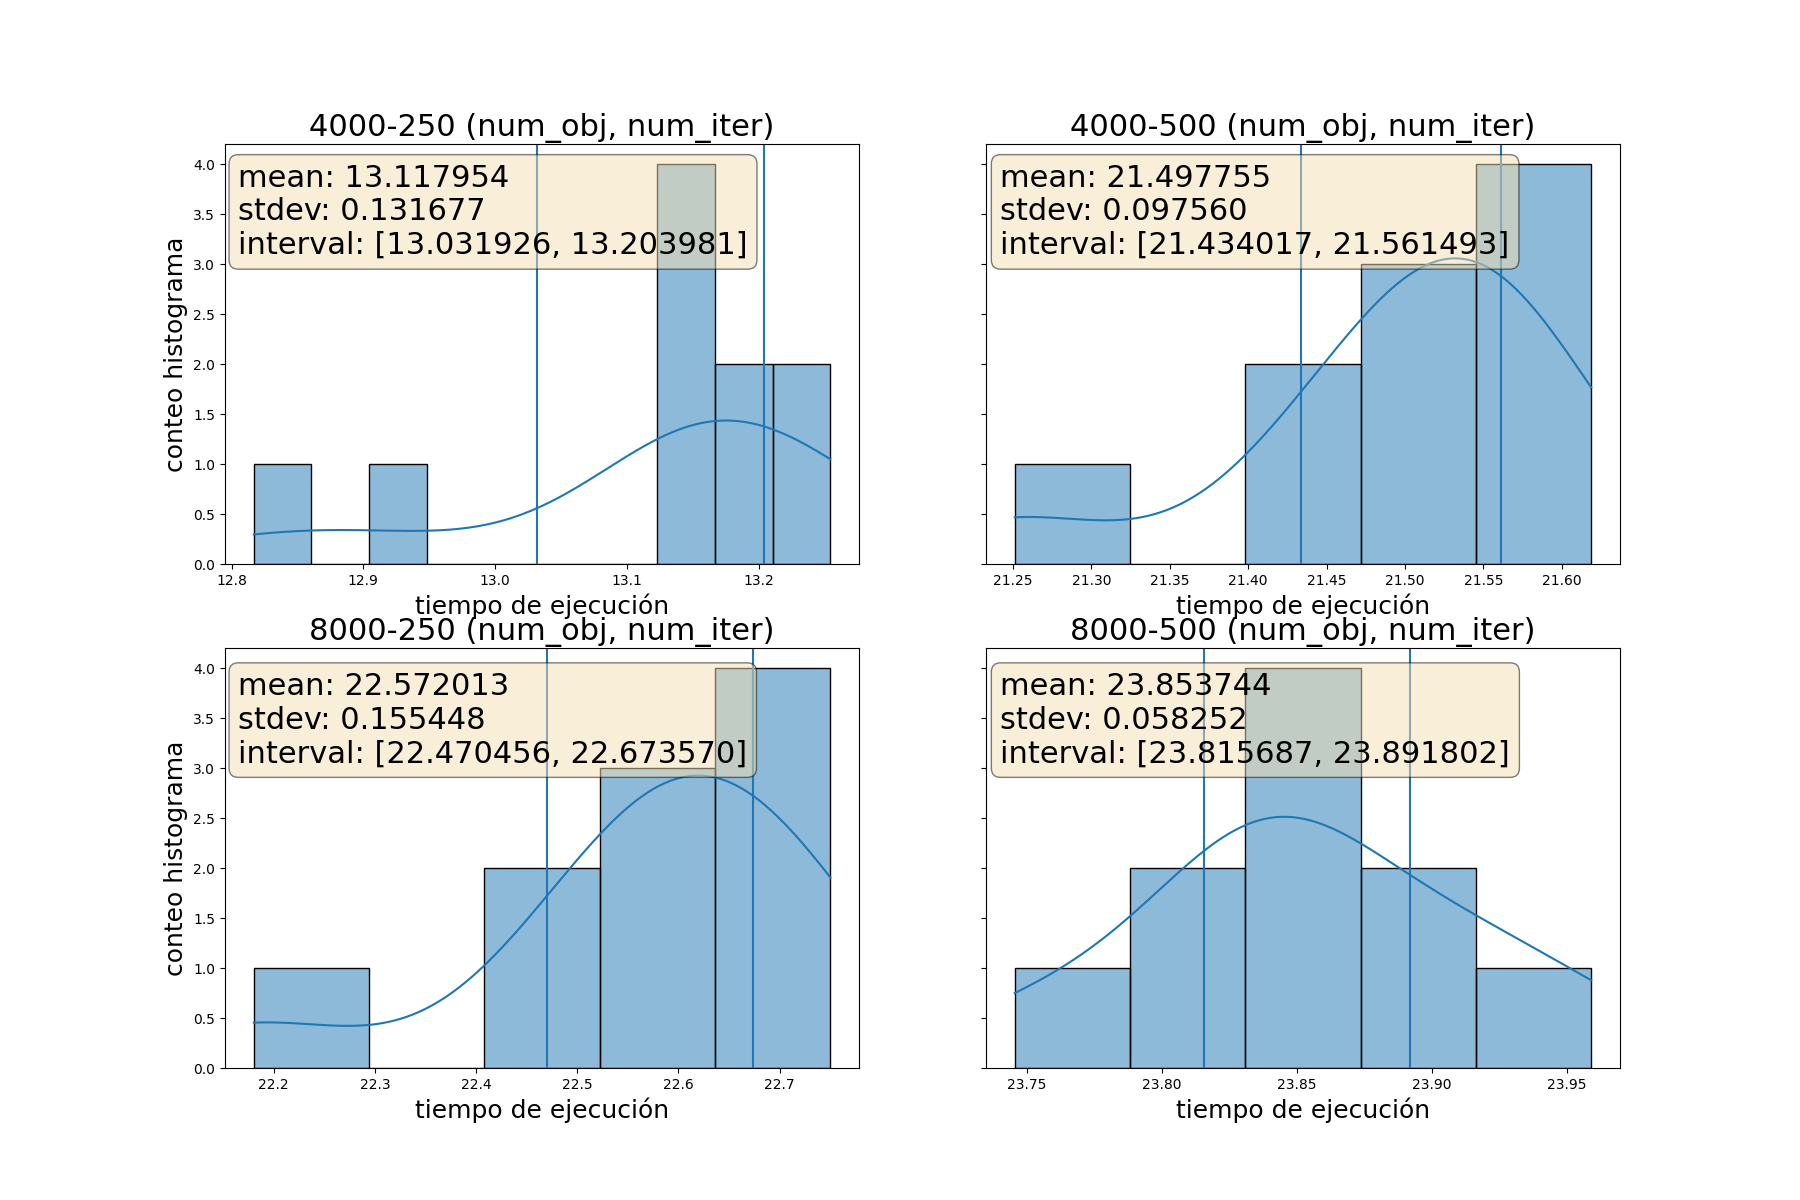
\includegraphics[width=0.8\linewidth,height=0.55\linewidth]{resources/p_1_samples_conf_interval.png}
		\label{fig:p_1}
	}%
	\caption{Pruebas con 8 hilos de ejecución y pruebas en algoritmo secuencial de la sección \ref{original}. SoA.}
	\label{fig:8core_p_1}
\end{figure}
\begin{figure}[htp]
	%\centering
	\hspace*{-3.5cm}
	\subfloat[Pruebas con 4 hilos de ejecución.]{%
		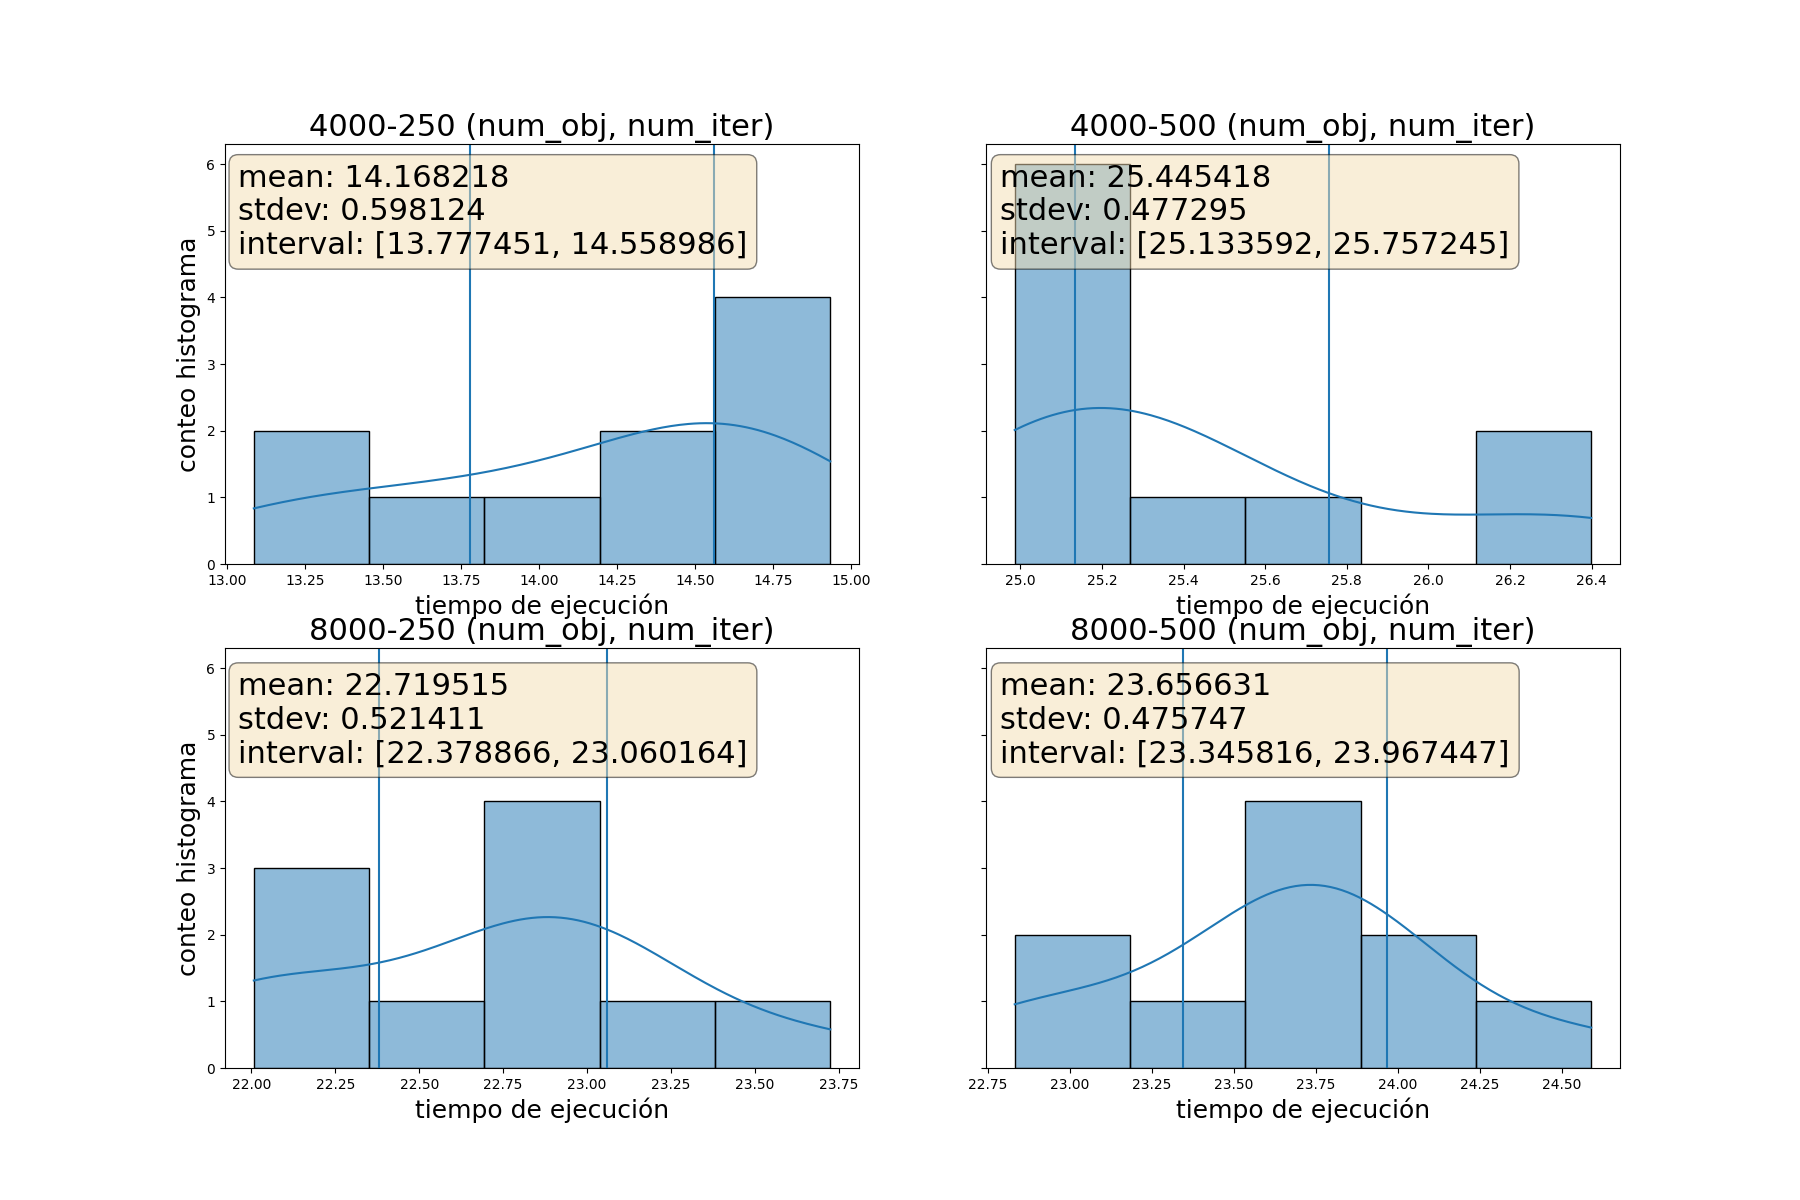
\includegraphics[width=0.8\linewidth,height=0.65\linewidth]{resources/4core_samples_conf_interval.png}
		\label{fig:4core}
	}%
	\subfloat[Pruebas con 16 hilos de ejecución.]{%
		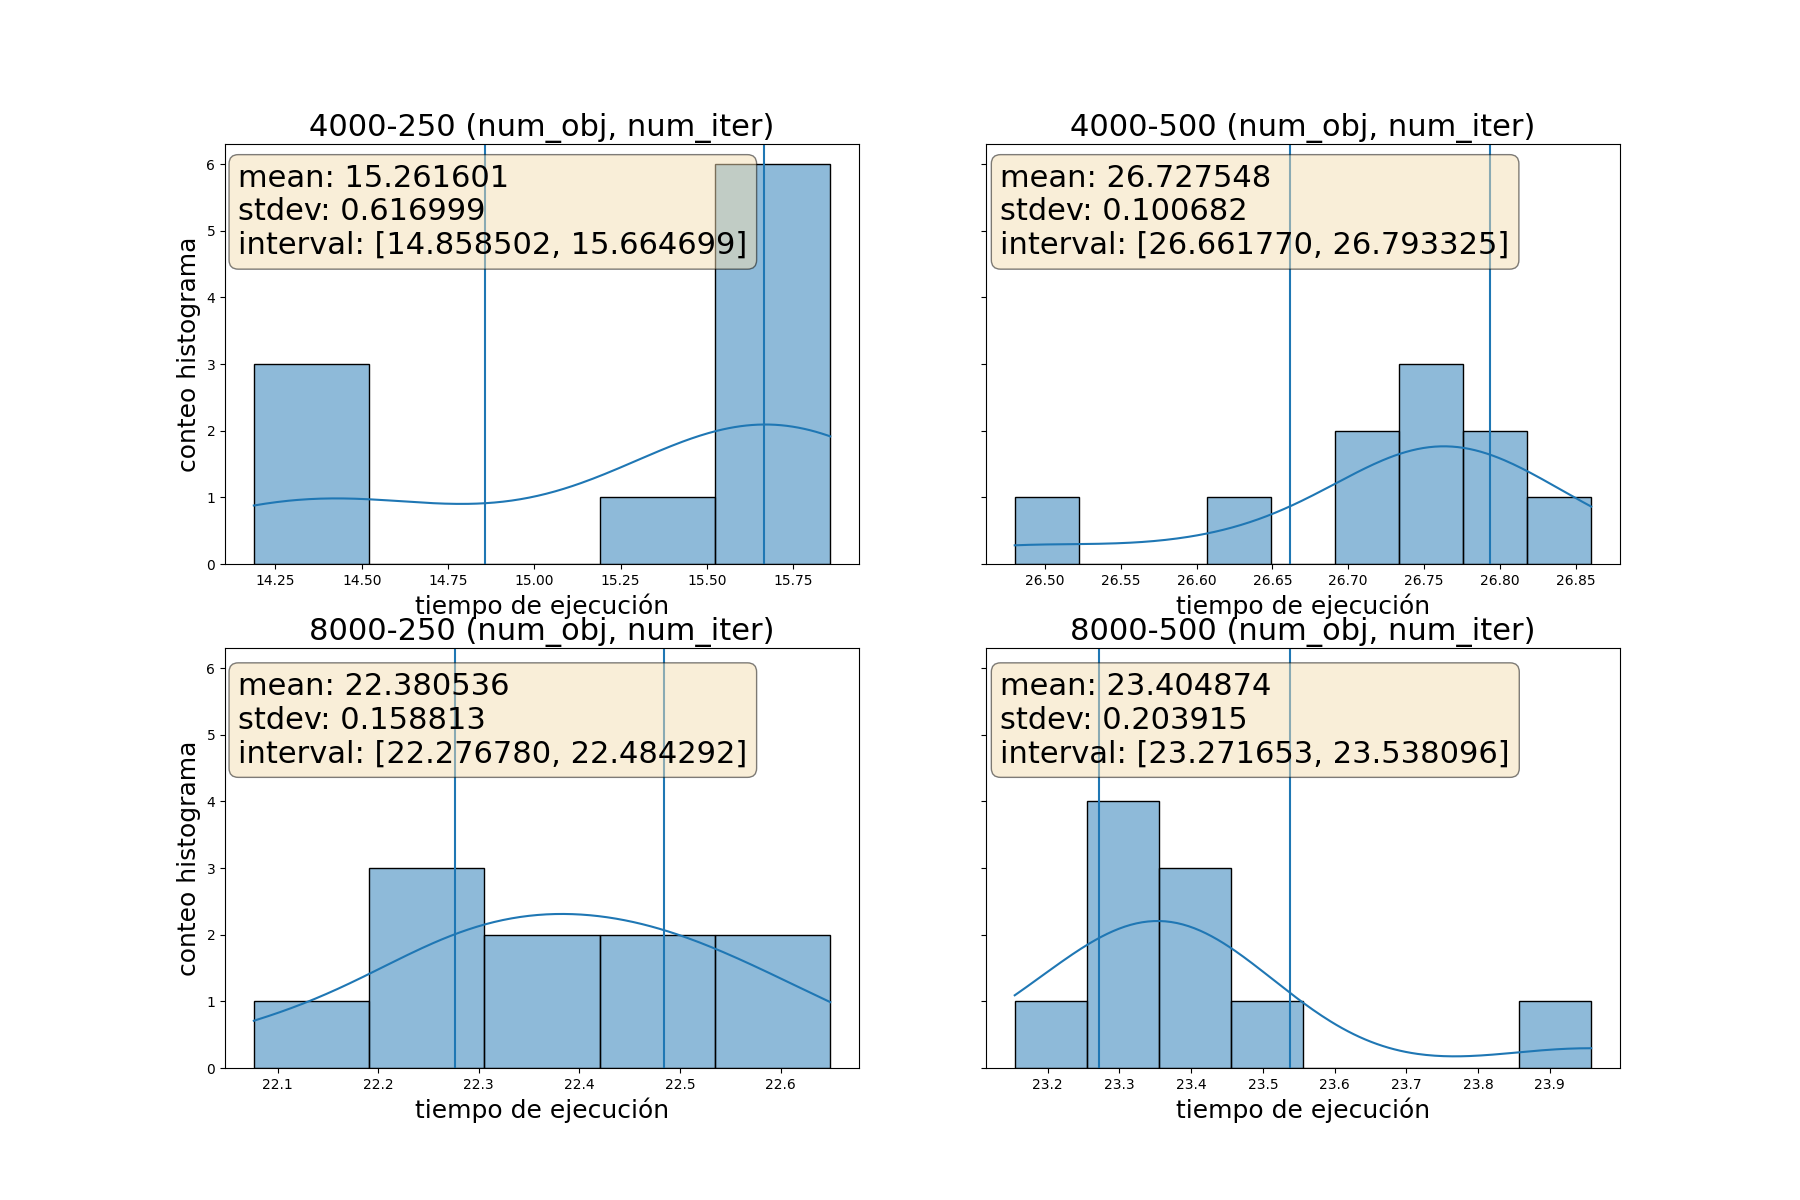
\includegraphics[width=0.8\linewidth,height=0.65\linewidth]{resources/16core_samples_conf_interval.png}
		\label{fig:16core}
	}%
	\caption{Pruebas con 4 y 16 hilos de ejecución. SoA.}
	\label{fig:4core_16core}
\end{figure}


Los resultados obtenidos en Kruskal-Wallis H-Test para las distintas configuraciones son:
\begin{itemize}
\item Configuración: num\_iterations: 4000, num\_objects: 250, p\_valor: 0.000000003707
	Sí hay \textbf{diferencia significativa} en las medias poblacionales.

\item Configuración: num\_iterations: 4000, num\_objects: 500, p\_valor: 0.000000000070
	Sí hay \textbf{diferencia significativa} en las medias poblacionales.

\item Configuración: num\_iterations: 8000, num\_objects: 250, p\_valor: 0.000000000481
	Sí hay \textbf{diferencia significativa} en las medias poblacionales.

\item Configuración: num\_iterations: 8000, num\_objects: 500, p\_valor: 0.000000000295
	Sí hay \textbf{diferencia significativa} en las medias poblacionales.
\end{itemize}
El bajo valor numérico de \textit{p\_valor} hace que para todas las configuraciones se rechace
la hipótesis nula ${H_0}$ de Kruskal-Wallis. Se concluye que hay una diferencia significativa
en los tiempos de ejecución.

Notar que 8 hilos de ejecución da la mejor performance del programa paralelo. El procesador
utilizado para las pruebas tiene 4 núcleos, que gracias a \textit{hyper-threading} de intel quedan en 8 hilos.
Entonces el programa que usa 8 hilos de ejecución es el que más aprovecha la configuración del hardware.
Tanto menos hilos (Figura \ref{fig:4core}) como más hilos (Figura \ref{fig:16core}) dan peores
resultados que los obtenidos en 8 hilos de ejecución (Figura \ref{fig:8core}).


\subsection{Secuencial vs. Paralelo.\label{t-test}}
En la sección \ref{opt_conclusiones} se habló de las dificultades que aparecieron al paralelizar el programa
original. Esto restringió mucho las optimizaciones aplicables sin modificar el resultado obtenido.
Como era de esperar, en \ref{fig:8core_p_1} podemos ver que el speedup no es la gran cosa. De hecho, nos urge
la necesidad de comprobar si de hecho hay un speedup.

Por ello en esta sección hacemos una prueba T-Test para
verificar si existe un speedup significativo (hipótesis alternativa) o si la velocidad de ejecución en realidad
es significativamente igual. La configuración paralela será la de 8 hilos de ejecución, porque entre los resultados
obtenidos, es la cantidad de hilos de ejecución candidata a mostrar un speedup significativo contra la versión secuencial.
\begin{displaymath}
\begin{cases}
	{H_0}: \mu_{8hilos} = \mu_{seq}\\
	{H_A}: \mu_{8hilos} \neq \mu_{seq}\\
\end{cases}
\end{displaymath}

Resultados T-Test para \textit{SoA}:

\begin{itemize}
\item Configuración: num\_iterations: 4000, num\_objects: 250, p\_valor: 0.000023486219
	Sí hay diferencia significativa en las medias de las muestras. \textbf{Favorece a secuencial.}\\
		$\mu_{seq} = 13.117954$, $\mu_{8hilos} = 14.397698$. $Speedup = 1.097557$

\item Configuración: num\_iterations: 4000, num\_objects: 500, p\_valor: 0.000000000000
	Sí hay diferencia significativa en las medias de las muestras. \textbf{Favorece a secuencial.}\\
		$\mu_{seq} = 21.497755$, $\mu_{8hilos} = 24.902056$, $Speedup = 1.158356$

\item Configuración: num\_iterations: 8000, num\_objects: 250, p\_valor: 0.000009911266
	Sí hay diferencia significativa en las medias de las muestras. \textbf{Favorece a 8 hilos.}\\
		$\mu_{seq} = 22.572013$, $\mu_{8hilos} = 21.050593$, $Speedup = 1.072274$

\item Configuración: num\_iterations: 8000, num\_objects: 500, p\_valor: 0.000000036031
	Sí hay diferencia significativa en las medias de las muestras. \textbf{Favorece a 8 hilos.}\\
		$\mu_{seq}: 23.853744$, $\mu_{8hilos}: 22.070424$, $Speedup = 1.080801$
\end{itemize}

Lo primero que se puede observar es que hay una diferencia significativa en cada prueba.
Esto significa que si hay un speedup, este es significativo, ya sea menor a 1 (más lento) o mayor a 1 (más rápido).

Los resultados nos muestran que el programa secuencial tiene un tiempo de ejecución levemente más rápido
para una cantidad medianamente grande de objetos (${N} <= 4000$). Pero la situación se revierte
en las pruebas donde ${N} = 8000$. Dificilmente esto se deba a mejoras en localidad de caché, ya que
como fue discutido en la sección \ref{opt_conclusiones}, poco se ha podido hacer en este ámbito.
Más bien, el speedup en muestras grandes se da porque el \textit{overhead} de creación
de procesos y sincronización (exigida para mantener el orden de operaciones), no se hace notar
si no hasta tamaños grandes de muestra.

\section{Conclusiones Finales.\label{conclusiones}}
En la paralelización de este programa nos encontramos con desafíos. Entre los cuales están: la asociatividad
del punto flotante, desafíos propios del paralelismo (), y decisiones en el algoritmo original descrito en
la sección \ref{original} que afectaron las optimizaciones factibles a la hora de paralelizar (como impocisiones
en el orden de operaciones). No obstante, para programas que procesan una gran cantidad de datos, como cuando ${num_objects=8000}$,
incluso el poco paralelismo que pudo ser aplicado mostró un speedup. Si bien para las pruebas realizadas este speedup no fue
muy grande, lo más probable es que la diferencia crezca a medida que la cantidad de datos lo haga.


Es crucial a la hora de paralelizar algoritmos, tener en cuenta la configuración del hardware. Queda demostrado
en la mejora de resultados al usar 8 hilos, o más bien, en los malos resultados obtenidos por 1, 2, 4, y 16 hilos (configuraciones
que no tienen en cuenta el hardware usado).


A su vez, la elección de estructuras de datos juega un gran papel al paralelizar algoritmos, e incluso al optimizar secuencialmente.
Empezando por lo `secuencial', SoA es mucho más apto a optimizaciones de vectorización, un \textit{trend} no menor en manufacturadores
de chips de hoy en día. A su vez, SoA en muchos casos, como el de este programa, se puede ajustar mejor a técnicas que mejoran
la localidad temporal y espacial.

A la hora de paralelizar, esta mejora en localidad de SoA se acentúa aún más. A diferencia de AoS, tener en caché únicamente
los datos necesarios para el cálculo, permite disminuir los fallos de caché al
facilitar la eliminación de \textit{cache-thrashing}. Es verdad que gran parte del desarrollo se concentró en SoA, en lugar de AoS, porque
desde el vamos parecía más optimizable por paralelismo y consideramos nos permitiría sacar mejores conclusiones para este proyecto (por
si nuestra inclinación por SoA no es evidente).

No descartamos que se hayan pasado por alto optimizaciones u otro tipo de consideraciones
en el diseño que podrían haber terminado en mejores resultados. Últimamente, la performance final se vió muy
afectada por decisiones en el diseño original. Se perdió la posibilidad de usar distintas optimizaciones
como consecuencia de priorizar la conservación del resultado final con respecto al programa inicial.

\printbibliography
\end{document}
